\documentclass[a4paper]{article}
\author{Chris Swetenham (s1149322)}
\title{IAML Assignment \\ \large Using Weka 3.6.2}
\date{November 22, 2011}

% \usepackage{fullpage}
\usepackage{verbatim}
\usepackage{enumerate}
\usepackage{graphics}
\usepackage{graphicx}
\usepackage{amsmath}
\usepackage{placeins}
\usepackage{subfigure}

\begin{document}

\maketitle

This assignment was discussed with Dan Mankowitz, Dino Vougioukas, Kostas Kanellis, Facundo Bellosi, Carlos Garc\'{\i}a.

\clearpage

\section*{Part A}

\subsection*{Question i}
Training on the dataset {\tt train\_faces.arff} and evaluating with 5-fold cross-validation, we evaluate three classifiers using their default settings: \\
\\
\begin{tabular}{lr}
Method & Accuracy \\
\hline
{\tt NaiveBayes} & 12\% \\
{\tt J48} & 37\% \\
{\tt SMO} & 46\%
\end{tabular}

\subsection*{Question ii}
We use the {\tt AddCluster} unsupervised attribute filter, using the EM algorithm, to add cluster labels to each training instance. We set the number of clusters to 10, corresponding to the 10 subjects in the dataset.
In the histogram for the resulting cluster attribute, shown in Figure~\ref{fig:a2img1}, we notice that there are two dominating clusters which with exactly 100 instances each. We were hoping to see 10 roughly equal clusters corresponding to the 10 subjects in the dataset. Additionally, labelling them by class, we see that there is very little correspondance between the two class and cluster attributes.

\begin{figure}[!htbp]
\centering
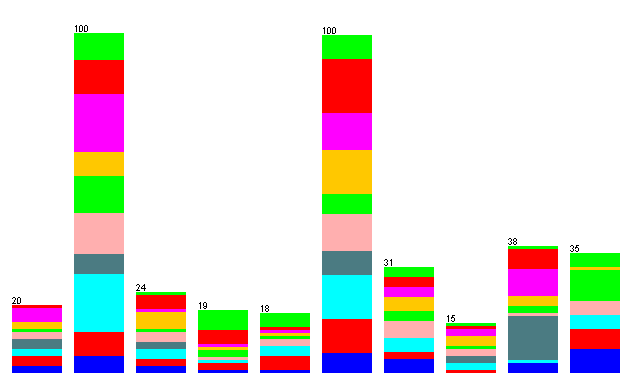
\includegraphics[width=0.8\textwidth]{A2-img1-clusters-cropped.png}
\caption{Cluster Histogram}
\label{fig:a2img1}
\end{figure}

\clearpage

Checking the histogram of the class labels, shown in Figure~\ref{fig:a2img2}, we notice that these are unevenly distributed, and further we have 400 instances rather than the 20*10 we were promised. The two dominating classes together sum to 200, the discrepancy between the expected and actual size of the dataset.

\begin{figure}[!htbp]
\centering
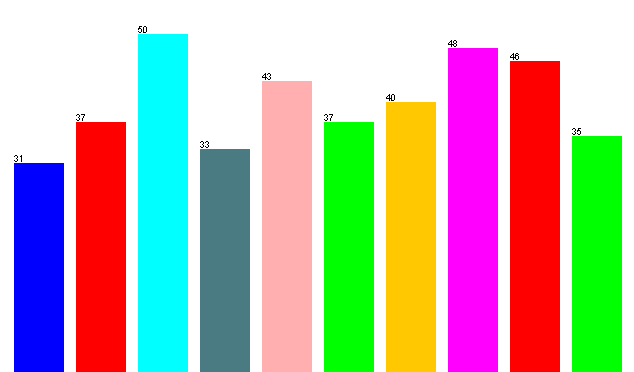
\includegraphics[width=0.8\textwidth]{A2-img2-classes-cropped.png}
\caption{Class Histogram}
\label{fig:a2img2}
\end{figure}

The dominating clusters are {\it cluster2} and {\it cluster6}. The first three images from each cluster are shown in Figure~\ref{fig:a2img3} and Figure~\ref{fig:a2img4}.

\begin{figure}[!htbp]
\centering
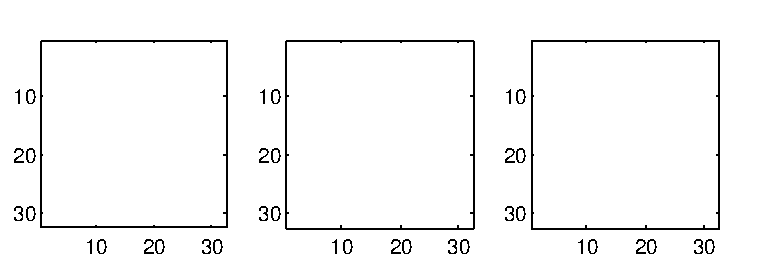
\includegraphics[width=0.8\textwidth]{A2-img3-cluster2-cropped.pdf}
\caption{cluster2, images 6, 12 and 20}
\label{fig:a2img3}
\end{figure}

\begin{figure}[!htbp]
\centering
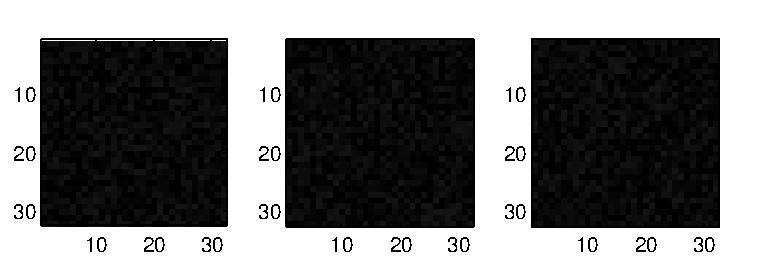
\includegraphics[width=0.8\textwidth]{A2-img4-cluster6-cropped.pdf}
\caption{cluster6, images 2, 15 and 29}
\label{fig:a2img4}
\end{figure}

\clearpage

The first three images from {\it cluster1} and {\it cluster3} are shown in Figure~\ref{fig:a2img5} and Figure~\ref{fig:a2img6}:

\begin{figure}[!htbp]
\centering
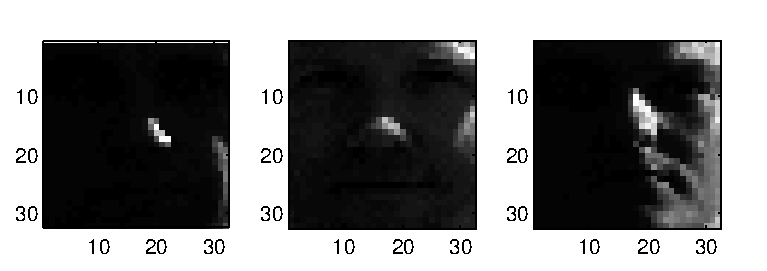
\includegraphics[width=0.8\textwidth]{A2-img5-cluster1-cropped.pdf}
\caption{cluster1, images 1, 7 and 8}
\label{fig:a2img5}
\end{figure}

\begin{figure}[!htbp]
\centering
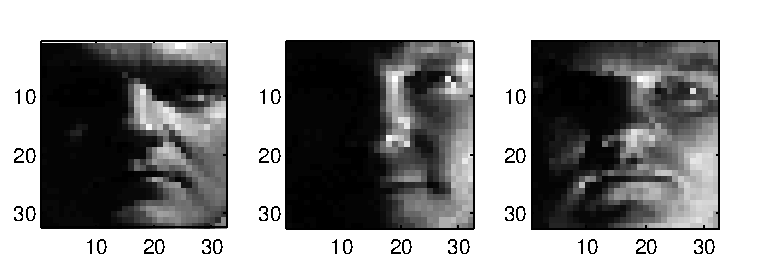
\includegraphics[width=0.8\textwidth]{A2-img6-cluster3-cropped.pdf}
\caption{cluster3, images 13, 17 and 19}
\label{fig:a2img6}
\end{figure}

We see that the two dominating clusters seem to be pure white and noisy dark images which are not relevant to our task.

% TODO include more discussion of how these bad instances affect the results in part A i). Consider cross-validation where we might have unbalanced subsets with a lot of the while or black images. Comment on each classifier?

% TODO SVM is sensitive to some outliers - if the dataset is not linearly spearable, misclassified instances become support vectors with a penalty and will affect the boundary

\subsection*{Question iii}
Using the filter {\tt RemoveWithAttribute}, we removed instances in {\it cluster2} and {\it cluster6}. As shown in Figure~\ref{fig:a3img1}, the resulting dataset has 20 instances of each class, as expected from the task description.
% 
\begin{figure}[!htbp]
\centering
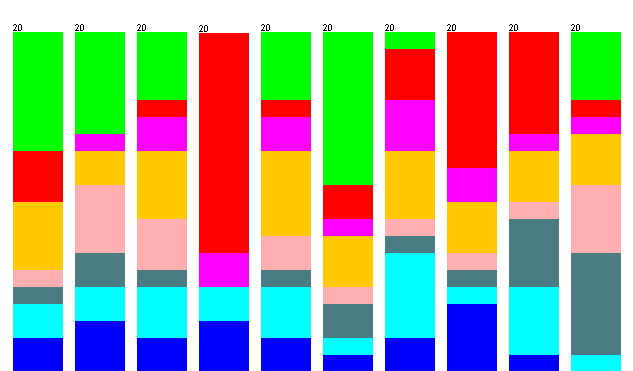
\includegraphics[width=0.7\textwidth]{A2-img3-remjunk-cropped.png}
\caption{Class Histogram after {\tt RemoveWithAttribute}}
\label{fig:a3img1}
\end{figure}

\subsection*{Question iv}
We remove the cluster attribute from the instances in the dataset, and as in part i) evaluate different methods with 5-fold CV:\\
\\
\begin{tabular}{lrr}
Method & Accuracy & Baseline \\
\hline
{\tt NaiveBayes} & 52.5\% & 12\% \\
{\tt J48} & 62\% & 37\% \\
{\tt SMO} & 88\% & 46\%
\end{tabular}\\
\\
We can compare this performance with the results from part i) as baseline. After removing the erroneous instances, the accuracy of all three classifiers has greatly improved. Since the dataset was smaller, the time taken to train and evaluate the classfiers was also shorter.

\subsection*{Question v}
We train the {\tt SMO} classifier from {\tt train\_faces\_clean.arff}, using {\tt val\_faces.arff} as test set.\\
\\
\begin{tabular}{lr}
Method & Accuracy \\
\hline
{\tt SMO} & 92\%
\end{tabular}\\
\\
This is comparable to the performance on the training data earlier. Two example correctly classified instances are shown in Figure~\ref{fig:a5img1}.

\begin{figure}[!htbp]
\centering
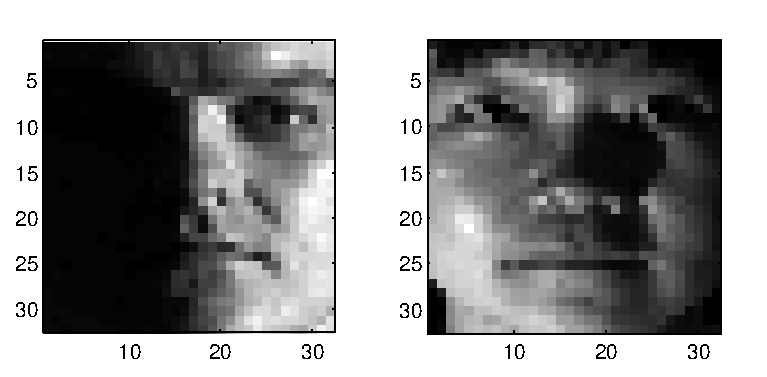
\includegraphics[width=0.8\textwidth]{A5-correct-cropped.pdf}
\caption{Correctly classified instances 32, 85}
\label{fig:a5img1}
\end{figure}

Two example incorrectly classified instances are shown in Figure~\ref{fig:a5img2}. The classifier seems to make mistakes on instances where the subject's eyes are entirely in shadow.

\begin{figure}[!htbp]
\centering
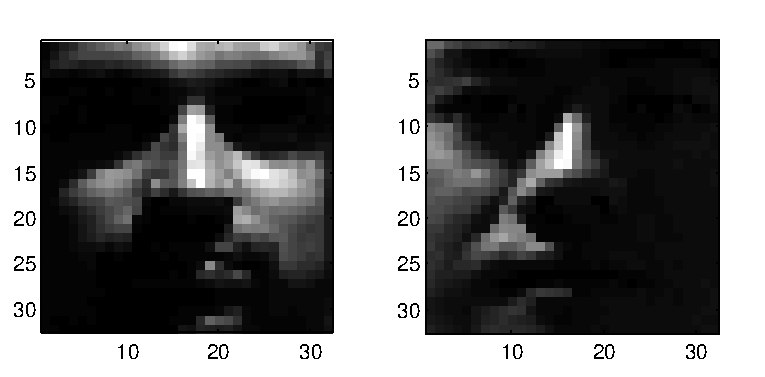
\includegraphics[width=0.8\textwidth]{A5-incorrect-cropped.pdf}
\caption{Incorrectly classified instances 15, 42}
\label{fig:a5img2}
\end{figure}

\FloatBarrier

\section*{Part B}
\subsection*{Question i}
In the Naive Bayes model, each of the attributes are independently distributed given the class label. This is not a very good assumption for our data set, since nearby pixels will usually have similar values, and lighting conditions affect pixels in similar ways across large regions of the image.

For continuous attributes, {\tt NaiveBayes} will build a gaussian distribution of the values for each pixel for each subject's images. This is a poor choice, because the many lighting conditions mean that the variation of any pixel within one class is much greater than the variation of that pixel between classes.

Discretization allows for more arbitrary distributions to be learned, for example we might have a bimodal distribution for a pixel with one mode when that pixel is in shadow and one when it is well lit. Choosing the number of bins is a parameterization problem; the more bins we allow, the closer fit to the data we allow, but the more parameters we have to learn. On one hand, we want to choose a small enough number of bins that we have some bins with multiple instances in them. On the other hand, too few bins will give us very little discriminative power.

After applying the unsupervised attribute filter {\tt Discretize} using different numbers of bins, we train {\tt NaiveBayes} and evaluate using 5-fold CV.\\
\\
\begin{tabular}{rr}
Bins & Accuracy\\
\hline
5 & 45\% \\
10 & 57\% \\
20 & 61.5\% \\
40 & 62\% \\
60 & 62.5\% \\
80 & 60.5\% \\
100 & 59\%
\end{tabular}\\
\\
Out of the settings tested, using 60 bins for discretization gives the best performance. We see a moderate gain in performance over the original NaiveBayes result (62.5\% vs 52.5\%); this is about what we would expect, since we improved on the original gaussian model, but {\tt NaiveBayes} remains less than ideal for the task at hand since its assumptions about the structure of the data do not hold well for our dataset.

\subsection*{Question ii}
{\tt InfoGainAttributeEval} works by computing the information gain of each attribute, which is the difference between the entropy of the marginal class distribution and the entropy of the class distribution conditioned on that attribute. The attribute with the highest information gain tells us the most about the class, and one with 0 information gain is independent of the class.

After removing the attributes with 0 information gain, 353 attributes were left - we note that the provided {\tt train\_faces\_clean\_best.arff} has 350 attributes.

\subsection*{Question iii}
As shown in Figure~\ref{fig:b3img1}, the selected pixels with highest information gain cluster around the areas of the eyes, the corner of the chin, and the mouth and nose, ignoring the cheeks and the nose bridge. This corresponds with the most distinguishing features of a human face.

A potential problem with the information gain criterion is that if we use it to select more than one feature at once, these features might be correlated, and so the second we select would tell us a lot by itself but very little if we already know the first.

\begin{figure}[!htbp]
\centering
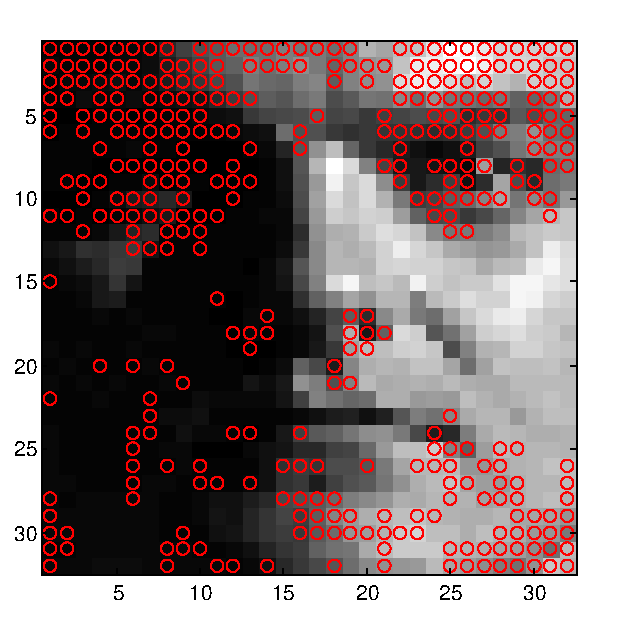
\includegraphics[width=0.8\textwidth]{B3-img1-pixels-cropped.pdf}
\caption{Pixels selected by {\tt InfoGainAttributeVal}}
\label{fig:b3img1}
\end{figure}

\FloatBarrier

\subsection*{Question iv}
We evaluate the same three classifiers as before on the new reduced dataset, again evaluating using 5-fold CV. We take the results from A iv) as baseline for comparaison.\\
\\
\begin{tabular}{lrr}
Method & Accuracy & Baseline \\
\hline
{\tt NaiveBayes} & 60\% & 52.5\% \\
{\tt J48} & 63.5\% & 62\% \\
{\tt SMO} & 91\% & 88\%
\end{tabular}\\
\\
We argued in part i) that the Naive Bayes algorithm has trouble with the original dataset due to the independence assumption being a poor fit to the data. Keeping only the attributes with the highest information gain should have removed a lot of attributes which were poor predictors and strongly correlated with each other, giving us better performance as observed.
% TODO - throwing away random pixels should be better than the original dataset, but doing it with information gain keeps better pixels.
The decision tree algorithm already works by selecting the attributes with the highest information gain, so as expected we see very little difference.

The SVM algorithm performs about the same as before. SVM should not be affected by additional attributes which are poor predictors.

\section*{Part C}
\subsection*{Question i}

The eigenvalues in descending order are plotted in Figure~\ref{fig:c1img1}. As we can see there is a sharp fall-off after the first few eigenvalues which contribute most of the variation in the dataset.

\begin{figure}[!htbp]
\centering
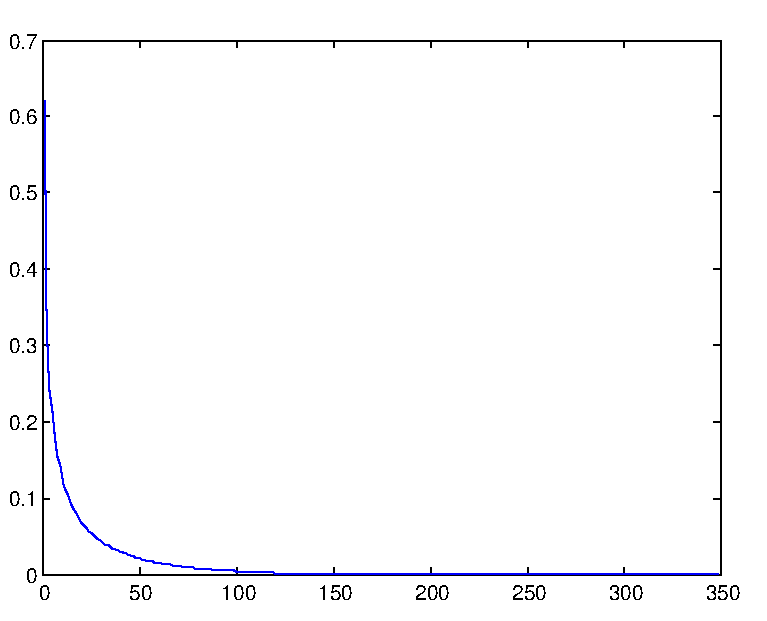
\includegraphics[width=0.8\textwidth]{C1-img1-eigenvalues-cropped.pdf}
\caption{Eigenvalues}
\label{fig:c1img1}
\end{figure}

\FloatBarrier

\subsection*{Question ii}

After using the {\tt PrincipalComponents} attribute filter to retain 95\% of the variation in the dataset, we are left with only 32 attributes.

We evaluate the same three classifiers as before on the new reduced dataset, again evaluating using 5-fold CV. We take the results from A iv) as baseline for comparaison.\\
\\
\begin{tabular}{lll}
Method & Accuracy & Baseline \\
\hline
{\tt NaiveBayes} & 81.5\% & 52.5\% \\
{\tt J48} & 61.5\% & 62\% \\
{\tt SMO} & 82.5\% & 88\%
\end{tabular}\\
\\
PCA gives us components which are uncorrelated and so suit {\tt NaiveBayes} well, and this is reflected in the improved performance of Naive Bayes on this version of the dataset.
% Uncorrelation guarantees indep. and correlation guarantees dep, but not hte other way around
The decision tree algorithm tries to find binary splits in the values of each attribute to classify instances. It is not affected by correlated attributes, since after it splits on one of them the inormation gain of the other would be small; so we would not expect an improvement. It would still be possible for the attributes we have thrown away to contain a lot of the information; the fact that we did not get worse performance suggests that most of the information is in fact contained in the principal components. 

Since PCA performs a rotation of the attribute space and SVM is a linear classifier, we would expect {\tt SMO} to perform as well on this dataset as on the original; if we perform the above evaluation but retain 100\% of the variation, we get an accuracy of 87.5\% using {\tt SMO} on the processed dataset. Therefore the attributes which had low variance and were discarded must have been useful for linear classification.

\subsection*{Question iii}

The eigenfaces corresponding to the largest eigenvalues capture gross detail, with successively finer features as one proceeds to smaller eigenvalues.

\begin{figure}[!htbp]
\centering
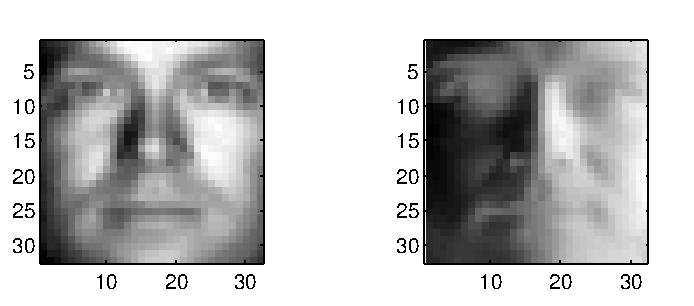
\includegraphics[width=0.8\textwidth]{C3-img1-eigfaces-cropped.pdf}
\caption{The first two eigenfaces}
\label{fig:c3img1}
\end{figure}

The largest two eigenvalues are 390.8 and 323.3. The corresponding eigenfaces are show in Figure~\ref{fig:c3img1}. These eigenfaces are an average face, corresponding to the variation in level of global illumination in the dataset, and a face which looks lit from the side, corresponding to the variation in left-right illumination in the images. Only when we get some number of eigenfaces in do we start seeing ones which distinguish between facial features as opposed to illumination; this makes sense since in the dataset the difference between images with different illumination directions is much more dramatic than the difference between two faces under the same illumination.

\FloatBarrier

\subsection*{Question iv}
Around 10 components are required to produce a face which is clearly recognisable as the original. As we increase the number of components, the face moves away from the average of the underlying faces and gains specific details from the face we are reconstructing.

\begin{figure}[!htbp]
\centering
\begin{center}
\subfigure{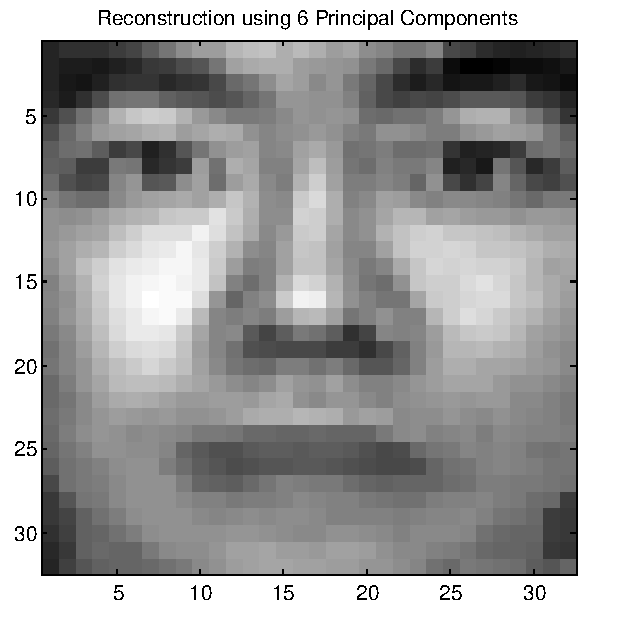
\includegraphics[width=0.4\textwidth]{C4-img6-6comp-cropped.pdf}}
\subfigure{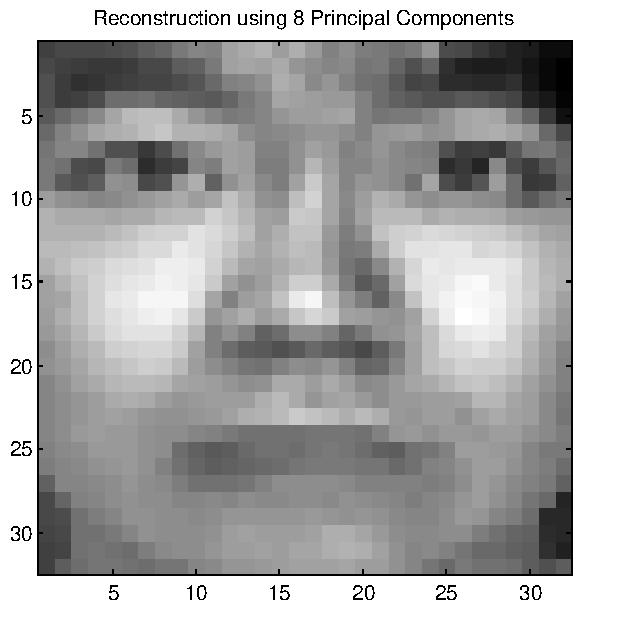
\includegraphics[width=0.4\textwidth]{C4-img2-8comp-cropped.pdf}}
\subfigure{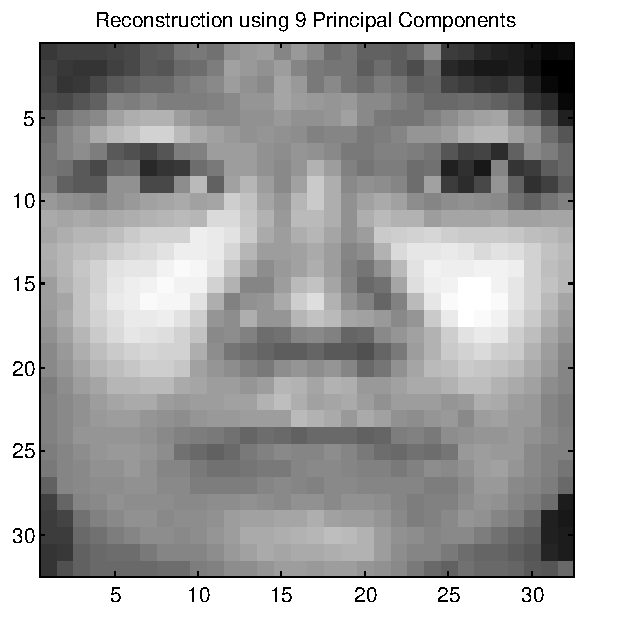
\includegraphics[width=0.4\textwidth]{C4-img3-9comp-cropped.pdf}}
\subfigure{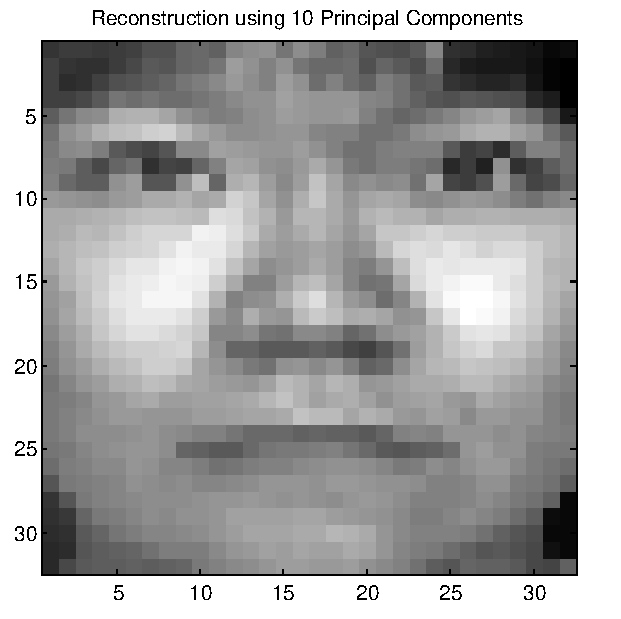
\includegraphics[width=0.4\textwidth]{C4-img4-10comp-cropped.pdf}}
\subfigure{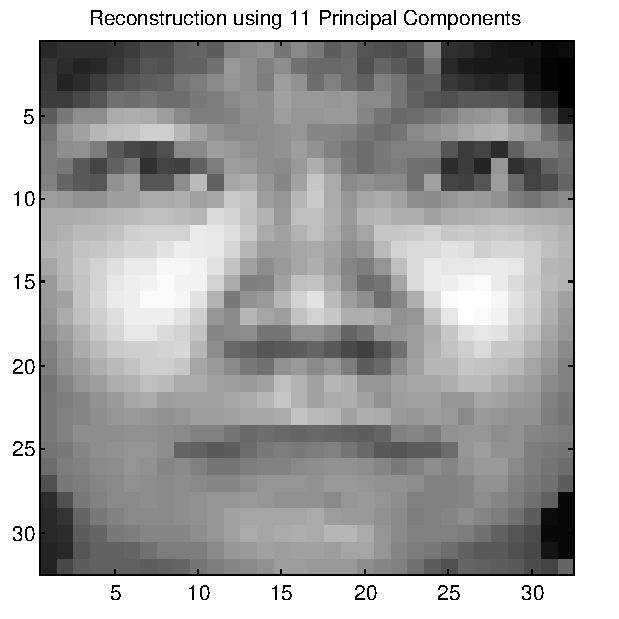
\includegraphics[width=0.4\textwidth]{C4-img5-11comp-cropped.pdf}}
\subfigure{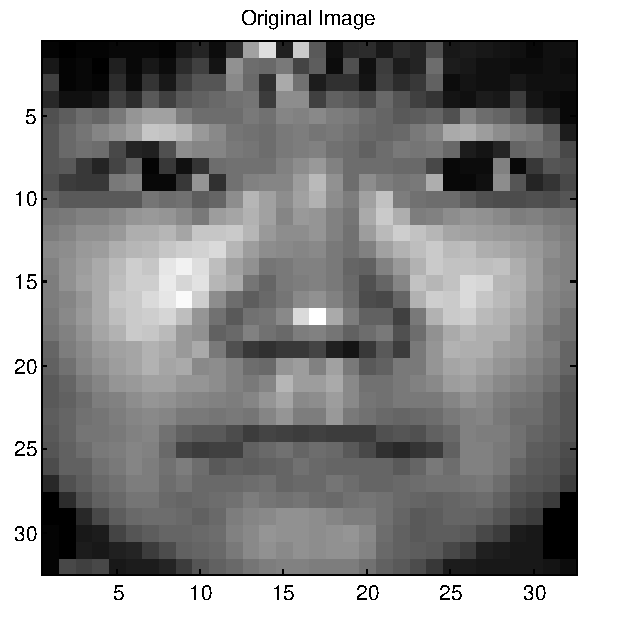
\includegraphics[width=0.4\textwidth]{C4-img1-orig-cropped.pdf}}
\end{center}
\caption{Reconstructing a face}
\label{fig:c4img1}
\end{figure}

\FloatBarrier

\subsection*{Question v}
We remove the four attributes with the largest eigenvalues, and evaluate the {\tt NaiveBayes} classifier using 5-fold CV, using the results from C ii) as baseline.\\
\\
\begin{tabular}{lll}
Method & Accuracy & Baseline \\
\hline
{\tt NaiveBayes} & 82.5\% & 81.5\% \\
\end{tabular}\\
\\
The accuracy has increased slightly. As stated before the greatest part of the variation in the dataset is in the lighting, which is not significant to our classification task; so the attributes we have left after removing the four with largest variation serve well for classifying the data.

\subsection*{Question vi}
We try running {\tt SMO} retaining different numbers of the top eigenfaces, evaluating the results using 5-fold CV. We include results obtained in part ii).\\
\\
\begin{tabular}{ll}
Eigenfaces & Accuracy \\
\hline
20 & 73.5\% \\
32 & 82.5\% \\
40 & 90\% \\
80 & 85\% \\
120 & 78\% \\
160 & 63\% \\
200 & 62.5\% \\
1024 & 87.5\% \\
\end{tabular}\\
\\
We notice that there is a peak in performance around 40 attributes, after which performance falls off; yet we know it climbs back up somewhere between 200 and 1024 attributes. This is difficult to explain. The peak at 40 attributes does not correspond to the 10 attributes after which a face becomes distinguishable by a human. As successively less important eigenfaces are kept, the level of detail we can distinguish increases, but the noise does as well. 

\section*{Part D}
\subsection*{Question i}

Results at 99\% confidence (95\% is identical), by dataset:

\begin{tabular}{lr|rrrr}
Dataset           & {\tt NaiveBayes} & {\tt J48} & & {\tt SMO} & \\
\hline
{\tt clean}       &            53.60 &     61.90 & &    88.00 &v\\
{\tt clean\_best} &            63.60 &     64.30 & &    90.10 &v\\
{\tt clean\_pca}  &            79.90 &     60.10 &*&    80.90 & \\
\hline
                  &           (v/ /*)&    (0/2/1)& &   (2/1/0)&
\end{tabular}\\
\\
We see that for two datasets, {\tt train\_faces\_clean} and {\tt train\_faces\_clean\_best}, {\tt SMO} does significantly better than {\tt NaiveBayes} with 99\% confidence.\\
\\
Results at 99\% confidence, by algorithm:\\
\\
\begin{tabular}{lr|rrrr}
Dataset          & {\tt clean} & {\tt clean\_best} & & {\tt clean\_pca} & \\
\hline
{\tt NaiveBayes} &       53.60 &             63.60 &v&            79.90 &v\\
{\tt J48}        &       61.90 &             64.30 & &            60.10 & \\
{\tt SMO}        &       88.00 &             90.10 & &            80.90 & \\
\hline
                 &      (v/ /*)&            (1/2/0)& &           (1/2/0)&
\end{tabular}\\
\\
We see that for {\tt NaiveBayes}, {\tt train\_faces\_clean\_best} and {\tt train\_faces\_clean\_pca} are both significantly better than {\tt train\_faces\_clean} with 99\% confidence. For {\tt J48}, none of the datasets are significantly better than the others.\\
\\
Based on this, I would select {\tt train\_faces\_clean\_best} for further experiments.
% train\_faces\_clean\_best?

\subsection*{Question ii}

We use the {\tt Randomize} instance filter to shuffle the dataset, using the default seed of 42. We then produce nested datasets by using the {\tt RemovePercentage} instance filter, setting {\tt invertSelection} true, with percentage values of 100 to 5. We evaluate the {\tt SMO} classifier on the resulting datasets, evaluating using {\tt val\_faces} rather than cross-validation.\\
\\
\begin{tabular}{lll}
Percentage & Instances & Accuracy\\
100\% & 200 & 92\% \\
80\% & 160 & 87\% \\
65\% & 130 & 86.5\% \\
50\% & 100 & 84\% \\
35\% & 70 & 76.5\% \\
10\% & 20 & 40\% \\
5\% & 10 & 21.5\%
\end{tabular}\\
\\
As we can see from the plot above, the performance is tailing off somewhat as we add more data, but the last 20\% of the dataset does provide a reasonable improvement and so a significantly larger dataset could still improve the performance of the classifier.

\subsection*{Question iii}
We use the {\tt FilteredClassifer} to allow us to use a validation set while performing filtering on the data. We train using {\tt train\_faces\_clean} and evaluate using {\tt val\_faces}. In one trial we apply PCA to the dataset and evaluate using {\tt NaiveBayes}. In the second trial we apply cluster lbels using the EM algorithm with the default seed of 100 and using 10 clusters, then apply PCA.\\
\\
\begin{tabular}{lr}
Filtering & Accuracy \\
PCA & 83.5\% \\
EM and PCA & 86.5\%
\end{tabular}\\
\\
Adding cluster labels has slightly helped. Although they don't contain any data independent of the original dataset, {\tt NaiveBayes} assumes all attributes are independent given the class labels, and so doesn't make use of all the information in the original dataset; by adding new features which are distinct from any of the original ones and which are useful in themselves for classification, we can improve the performance of the classifier.

% TODO: Try the Vote meta-classifier with multiple methods.
% TODO: Expected J48 do do very well after PCA because it should give us independent attributes, which will then have independent information gains! 
% TODO: PCA gives us attributes which are marginally independent. NaiveBayes assumes attributes which are conditionally independent, given the class. Decision trees assume/do well with...data that is separable along attribute axes? SVM needs data that is (mostly) linearly separable.

\section*{Part E}

Using both the {\tt train\_faces\_clean} and {\tt train\_faces\_clean\_best}, we systematically explored combinations of the techniques and classifiers used in previous parts, trying to improve on the 92.5\% rate obtained with {\tt SMO} on the {\tt best} dataset. The only success was found when applying PCA retaining 100\% of variation, ranking the resulting attributes by information gain, removing all those with 0 information gain, and adding a cluster label using EM with 10 clusters before classifying with {\tt SMO}; this gave 93\% accuracy. Unfortunately applying clustering after PCA gives an error in WEKA, even when telling it to ignore the class label using the ignoredAttributes field, so this technique could not be applied to the test set. Finally, we tried different classifiers with cool-sounding names until we hit upon {\tt MultilayerPerceptron} which gives 96.5\% on {\tt val\_faces\_best}. These results and the test set predictions are included in the file {\tt iaml\_assignment.res} submitted alongside this report.

\end{document}
